Las gráficas indican la tarifa de internet de dos compañías telefónicas.

\begin{figure}[H]
    \centering
    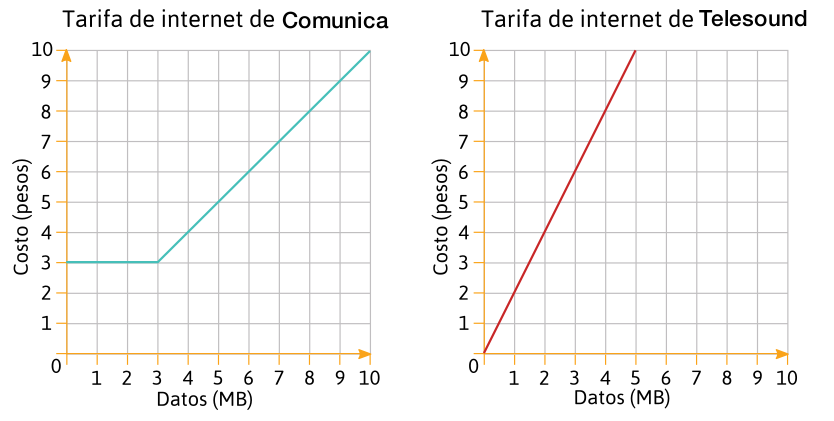
\includegraphics[width=0.8\linewidth]{../images/companias_telefon}
\end{figure}

\begin{multicols}{2}
    \begin{parts}
        \part ¿Cuál de las dos compañías tiene una tarifa inicial de 3 pesos por los primeros 3 MB?

        \begin{solutionbox}{1.2cm}
            Comunica.
        \end{solutionbox}

        \part ¿Cuál de las dos compañías ofrece la tarifa más alta después de los 3 MB?

        \begin{solutionbox}{1.2cm}
            Telesound.
        \end{solutionbox}
        \columnbreak
        \part ¿En cuál de las dos compañías la relación entre el costo y la cantidad de datos es una variación proporcional?

        \begin{solutionbox}{1.2cm}
            Telesound.
        \end{solutionbox}

        \part ¿Qué características de la gráfica representa una variación proporcional entre el costo y la cantidad de datos?

        \begin{solutionbox}{1.6cm}
            La gráfica es una recta que pasa por el origen del plano.
        \end{solutionbox}
    \end{parts}
\end{multicols}
